\documentclass[../main.tex]{subfiles}
\begin{document}

\chapter{Manejo de fauna y biodiversidad}

La huerta es un sistema vivo. Esto que significa que, como en todo sistema donde hay organismos vivos, se relacionarán entre ellos y buscarán un equilibrio para que todos puedan adquirir los recursos para sobrevivir y persistir en el tiempo y espacio. \\

Por lo que es importante tener una visión de nuestra huerta como un gran organismo vivo o un pequeño ecosistema autosustentable. \\

Nuestra labor consiste en \tcbox{acompañar a la naturaleza}, no combatirla.

Las tareas que llevemos a cabo tienen que enfocarse en la prevención, no en la reparación.\\

\begin{recuadroV}
    Prevenir implica que para poder evitar que el daño por insectos llegue a afectar la producción de nuestras plantas en la huerta es necesario llevar adelante labores que permitan el buen crecimiento de las plantas y las fortalezcan. De esta manera, podrán defenderse eficientemente del ataque de insectos y enfermedades.
\end{recuadroV}



\section{La fauna y su interacción con la huerta}

En la naturaleza las plantas se encuentran dispuestas de una manera desordenada o heterogénea en el espacio, y no están organizadas y concentradas como en una huerta. Su disposición natural y otros factores hacen que las poblaciones de insectos y plantas se auto-regulen. \\

Si fuéramos insectos veríamos a una huerta como un gran festín, donde todo el alimento está servido para nosotros y es fácil acceder a él. Aún bajo esa perspectiva, no todo insecto presente será una plaga; hay una variedad de bichos que podemos encontrar en nuestra huerta que no dañan nuestras plantas al punto de limitar su producción, e incluso hay otros insectos que no causarán daño alguno, siendo benéficos. \\

\hfill\\

\begin{recuadroV}
    Es muy importante conocer los insectos, saber quiénes son, y qué hacen en nuestra huerta. Este conocimiento nos ayudará a comprender mejor su interacción y que cuando alguna especie de insecto se vuelve plaga (lo cual implica representar una fuerza que reduzca la producción o eficiencia de las plantas) es porque existe un desequilibrio en nuestro sistema-huerta.
\end{recuadroV}

\begin{wrapfigure}[15]{i}[0cm]{0.65\textwidth}
    \centering
    \begin{tikzpicture}
        \def\ig{%
         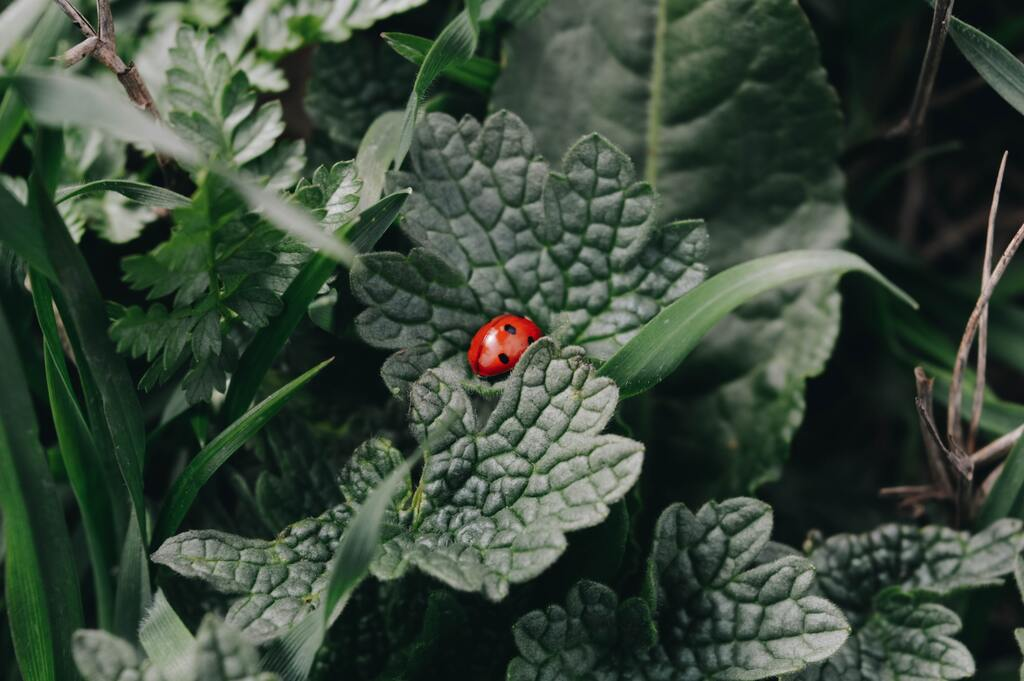
\includegraphics[width={0.6\textwidth},keepaspectratio]{insectos/7.jpg}}
       \node [inner sep=0pt](image) at (0,0) {\phantom{\ig}};
       \clip[rounded corners=5mm] ($(image.south west)+(\bord,\bord)$) rectangle ($(image.north east)-(\bord,\bord)$);
       \node[inner sep=0pt](image) at (0,0) {\ig};
      \end{tikzpicture}
    \caption*{\color{CompostGreen!50!black}Muchos bichitos colaboran con nuestra misión}
    \label{tutoraje1}
\end{wrapfigure}

Intercalando distintos tipos de plantas podemos más fácilmente mantener y promover el equilibrio de nuestro sistema-huerta. Una vía para manejar el entorno de esta manera es cultivando plantas aromáticas, como ser salvia, romero, orégano, menta, ruda, albahaca, flores como caléndulas o copetes.

Otra manera es dejar florecer algunas plantas que atraen insectos benéficos para la huerta, por ejemplo apio, brócoli, hinojo, perejil y acelga.

La ortiga es una buena compañera, ya que actúa como planta huésped de insectos aliados, a la vez, con sus hojas puede preparar una solución que previene el ataque de las posibles plagas.

El ajo también puede ayudarnos con las posibles plagas, y lo podemos aprovechar para preparar soluciones insecticidas.



\section{¿A quienes podemos encontrarnos en nuestra huerta?}


Alguna parte de la fauna que nos ayuda a controlar nuestra huerta es microscópica y podemos encontrarla como parte del suelo. Esta parte es muy importante para la prosperidad de nuestra huerta, pero no es lo único que participa. \\

\subsection{Quienes pueden ayudarnos con nuestras tareas}

\subsubsection{Vaquitas}

\begin{figure}[H]
    \centering
    \begin{tikzpicture}
        \def\ig{%
         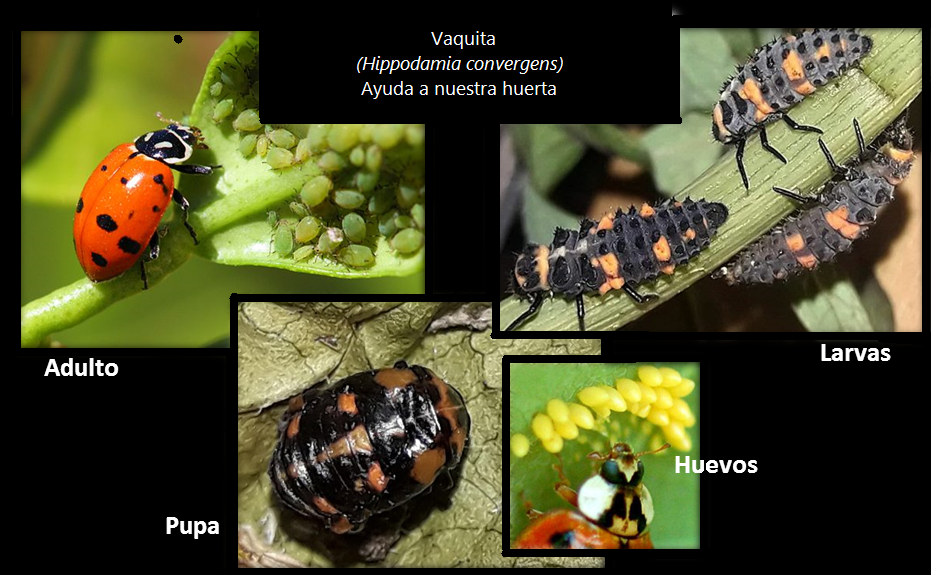
\includegraphics[width={\textwidth},keepaspectratio]{insectos/1.png}}
       \node [inner sep=0pt](image) at (0,0) {\phantom{\ig}};
       \clip[rounded corners=5mm] ($(image.south west)+(\bord,\bord)$) rectangle ($(image.north east)-(\bord,\bord)$);
       \node[inner sep=0pt](image) at (0,0) {\ig};
      \end{tikzpicture}
      \begin{tikzpicture}
        \def\ig{%
         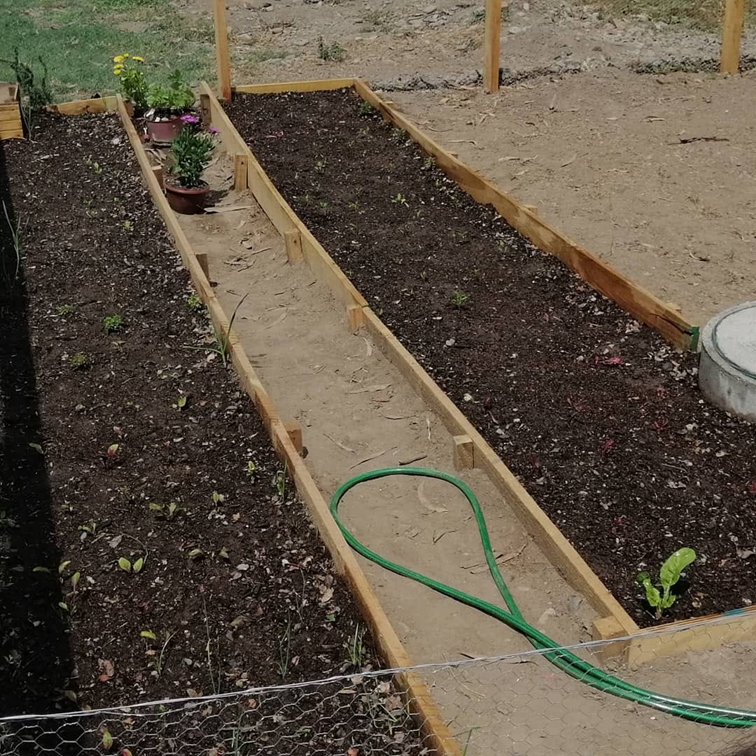
\includegraphics[width={\textwidth},keepaspectratio]{insectos/2.png}}
       \node [inner sep=0pt](image) at (0,0) {\phantom{\ig}};
       \clip[rounded corners=5mm] ($(image.south west)+(\bord,\bord)$) rectangle ($(image.north east)-(\bord,\bord)$);
       \node[inner sep=0pt](image) at (0,0) {\ig};
      \end{tikzpicture}
    \caption*{\color{CompostGreen!50!black}Las vaquitas, aliadas de nuestra huerta}
    \label{insectos1}
\end{figure}

\subsubsection{Crisopas}

Un importante benefactor para nuestros plantines son las Crisopas. Sus larvas son predadores de ácaros, pulgones y otros organismos indeseables. Por su parte, los adultos son polinizadores, lo que significa que ayudan a las plantas a reproducirse. 
Sus huevos son muy llamativos, tienen un filamento que los eleva de la superficie del suelo, protegiéndose de ser consumidos por otros insectos. 
En el caso de las crisopas pardas, sus huevos no tienen este filamento, por lo cual a veces aprovechan los pelitos de las hojas para colocar los huevos sobre ellos.

\begin{figure}[H]
    \centering
    \begin{tikzpicture}
        \def\ig{%
         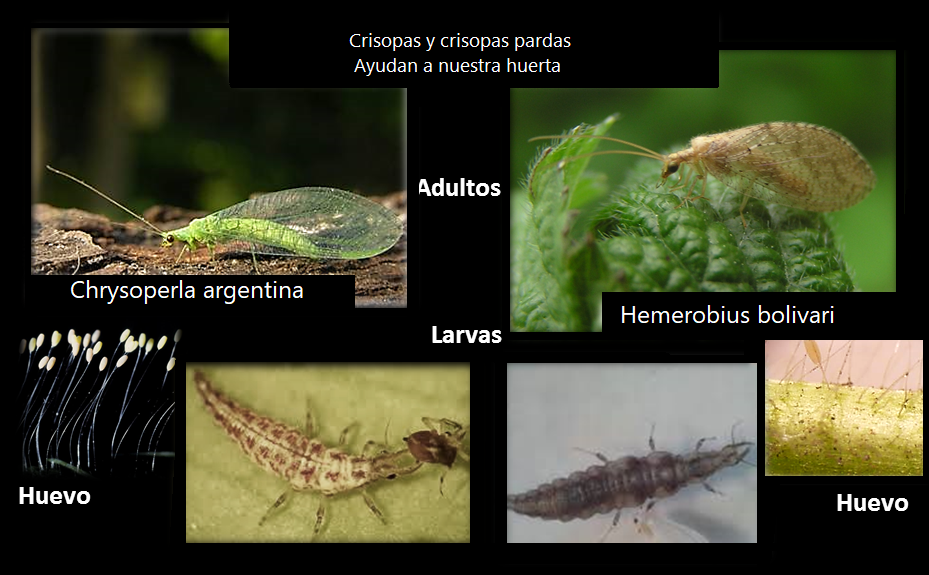
\includegraphics[width={0.9\textwidth},keepaspectratio]{insectos/3.png}}
       \node [inner sep=0pt](image) at (0,0) {\phantom{\ig}};
       \clip[rounded corners=5mm] ($(image.south west)+(\bord,\bord)$) rectangle ($(image.north east)-(\bord,\bord)$);
       \node[inner sep=0pt](image) at (0,0) {\ig};
      \end{tikzpicture}
    \caption*{\color{CompostGreen!50!black}Las crisopas, aliadas de nuestra huerta}
    \label{insectos2}
\end{figure}

\subsubsection{Otras vaquitas, mamboretás, libélulas, avispitas y abejas}

\begin{figure}[H]
    \centering
    \begin{tikzpicture}
        \def\ig{%
         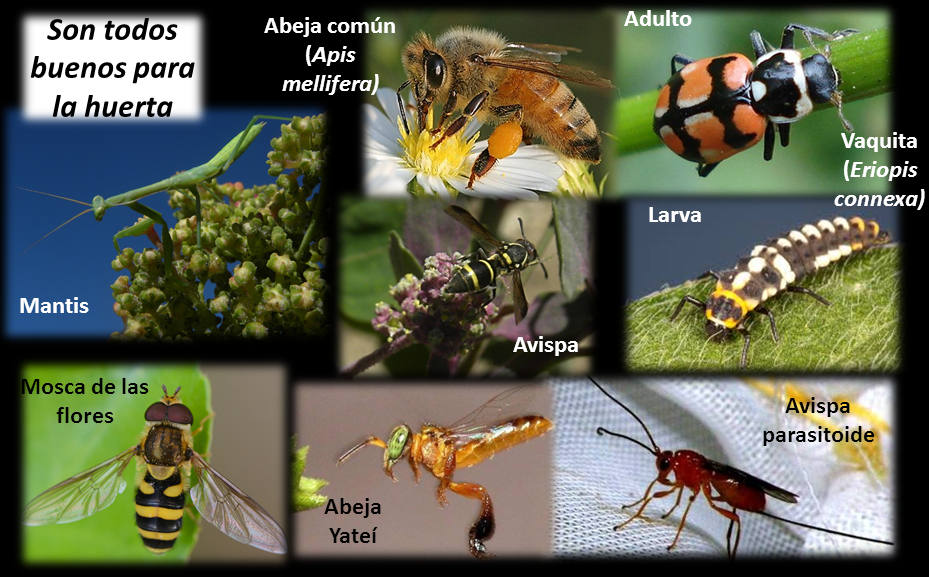
\includegraphics[width={0.9\textwidth},keepaspectratio]{insectos/4.png}}
       \node [inner sep=0pt](image) at (0,0) {\phantom{\ig}};
       \clip[rounded corners=5mm] ($(image.south west)+(\bord,\bord)$) rectangle ($(image.north east)-(\bord,\bord)$);
       \node[inner sep=0pt](image) at (0,0) {\ig};
      \end{tikzpicture}
    \label{insectos3}
\end{figure}

La mantis, las vaquitas y algunas larvas de moscas nos ayudan siendo depredadores de otras potenciales plagas. Las avispas parasitoides ponen huevos en el cuerpo de otros insectos para que los nuevos individuos se desarrollen en su interior, controlando las plagas. \\

Las abejas y avispas colaboran con la polinización de las plantas.\\

\subsection{Quienes pueden convertirse en plagas}

Bicho moro, ácaros, langostas, gusanos, cochinillas, orugas, chinches, pulgones vaquitas de San Antonio

\begin{figure}[H]
    \centering
    \begin{tikzpicture}
        \def\ig{%
         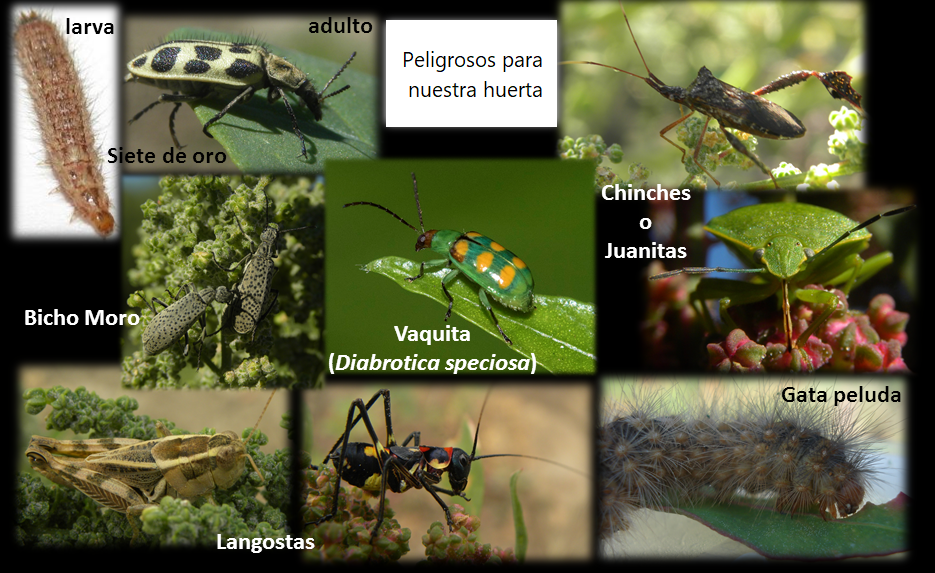
\includegraphics[width={\textwidth},keepaspectratio]{insectos/5.png}}
       \node [inner sep=0pt](image) at (0,0) {\phantom{\ig}};
       \clip[rounded corners=5mm] ($(image.south west)+(\bord,\bord)$) rectangle ($(image.north east)-(\bord,\bord)$);
       \node[inner sep=0pt](image) at (0,0) {\ig};
      \end{tikzpicture}
      \begin{tikzpicture}
        \def\ig{%
         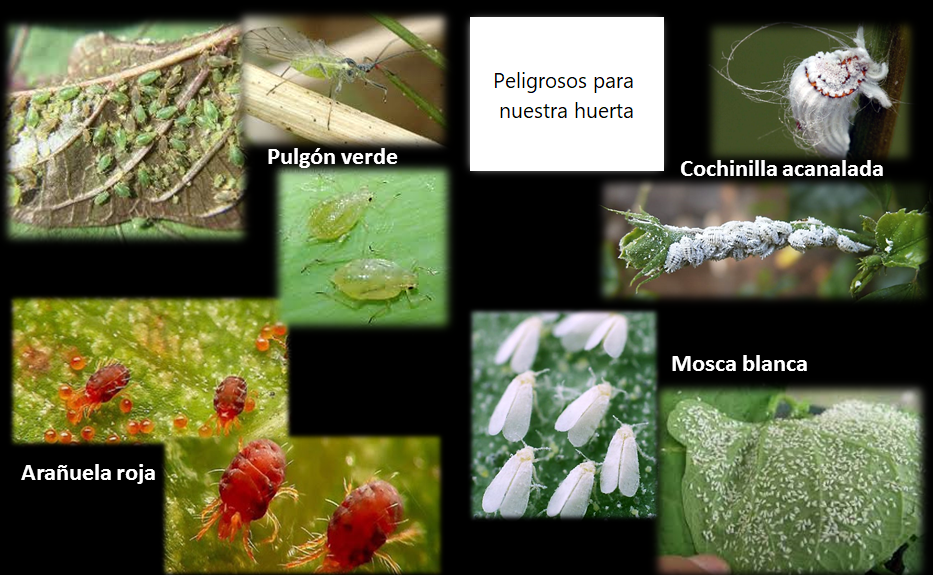
\includegraphics[width={\textwidth},keepaspectratio]{insectos/6.png}}
       \node [inner sep=0pt](image) at (0,0) {\phantom{\ig}};
       \clip[rounded corners=5mm] ($(image.south west)+(\bord,\bord)$) rectangle ($(image.north east)-(\bord,\bord)$);
       \node[inner sep=0pt](image) at (0,0) {\ig};
      \end{tikzpicture}
    \caption*{\color{CompostGreen!50!black}Pueden convertirse en plagas y afectar nuestra huerta}
    \label{insectos4}
\end{figure}

Las larvas del siete de oro, las chinches y la vaquita que consumen la savia de la planta, los cortadores de hojas como las larvas de mariposa, como las gatas peludas, y las langostas, son plagas que pueden amenazar nuestro cultivo.\\

Otros individuos pueden causar daño son los pulgones, arañuelas (ácaros) y moscas blancas. También consumen la savia y los fluidos celulares de las plantas, principalmente de las hojas, y son importantes transmisores de enfermedades a las plantas. Se los distingue porque siempre se encuentran agrupados sobre la superficie de las hojas (o en la parte de atrás), tallos y flores.

\vfill

\pagebreak

\end{document}